\setcounter{secnumdepth}{0}

\chapter{Shika Express Demonstrations for Physics}

\section{Egg Float}

\begin{description*}
\item[Topic:]{Density/Relative Density (Form 1)}
\item[Materials:]{2 fresh eggs, 2 containers (bottles cut in half), salt (less than half a cup)}
\item[Setup:]{Fill two containers with water and place a fresh egg in each. }
\item[Procedure:]{Leave one as it is and add salt to the other. Add and mix salt until the egg floats in the saltwater container.}
%\item[Hazards:]{}
\item[Questions:]{Why does the egg float in saltwater but sink in fresh water?}
\item[Theory:]{Saltwater has a greater density than fresh water. A fresh egg has a density between fresh water and saltwater. Since an egg is denser than freshwater, it sinks. Since an egg is less dense than saltwater, it floats.}
\item[Applications:]{This is the same reason why it is easier to stay afloat when swimming in the ocean (saltwater) as opposed to a lake (fresh water).}
%\item[Notes:]{}
\end{description*}

\begin{center}
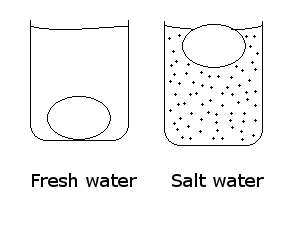
\includegraphics[width=5cm]{./img/egg-float.png}
\end{center}


\section{Pressure in a Bottle}

\begin{description*}
\item[Topic:]{Pressure (Form 1)}
\item[Materials:]{1.5 L bottle, syringe needle or pin/nail, water}
\item[Setup:]{Use a syringe needle, heated nail, etc. to poke three holes into a bottle. Put one hole near
the bottom, one near the middle, and the last hole between them.}
\item[Procedure:]{Fill the bottle with water and place on a table. Observe the trajectories of water coming from the three holes.}
%\item[Hazards:]{}
\item[Questions:]{}\hfill
\begin{enumerate*}
\item What do you notice about the trajectory of the water from each hole? Which one reaches the furthest horizontal distance?
\item How does the pressure change with the depth of the water? Why?
\end{enumerate*}
\item[Theory:]{The water flowing from the lower holes follows a shallower arc and hits the ground further from the bottle. The added weight of the water above the lower holes increases the pressure, resulting in an increased initial horizontal velocity. The relationship that pressure increases with depth is shown. ($P = \rho g h$)}
\item[Applications:]{The wall of a dam is made much thicker at the bottom than at the top. Also, water storage tanks are placed at the top of a building. This is because the pressure in a liquid is related to its depth.}
\item[Notes:]{There is a difference between depth and height. Height is measured from the reference point upward while depth is measured from the reference point downward. The reference point in this case is at the surface of water.}
\end{description*}

\begin{center}
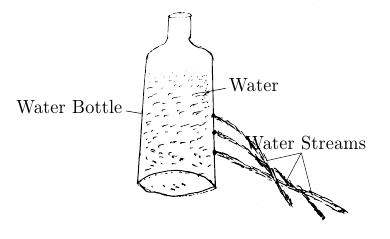
\includegraphics[width=8cm]{./img/pressure-liquid-alt.png}
\end{center}

%\begin{figure}
%\begin{center}
%\def\svgwidth{150pt}
%\chapter{Pressure within a Liquid}

\section{Aim}
To examine the relationship between the depth and the pressure within a liquid

\section{Background Information}
If you place a weight on your shoulders you will feel a pain which means the pressure on your body has increased. Therefore, if you were to enter into a liquid, like a lake, so that there is some liquid above you, you might think that the pressure on your body should change. Pressure in liquids is a very important topic for things like domestic water systems and dam construction. Thus, a student should find out if there is some relationship between the depth in a liquid and the pressure in the liquid at that depth, to better understand these observations. 

\section{Materials}
Tall jar can, water, bucket, 3 rubber tubes of equal length and diameter as the holes, 3 clips.

\section{Procedure}
\begin{enumerate}
\item Plug the holes of the Tall jar with rubber tubes and close the tubes with clips.
\item Fill the jar with water and then open the tubes one after the other starting with the top one.
\item Observe from each tube, how far the water travels before hitting the ground. 
\end{enumerate}

\begin{figure}[h!]
\centering
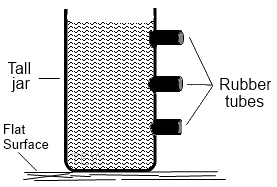
\includegraphics[width=8cm]{./img/pressure-liquid-1.png}
\caption{Pressure within a Liquid practical setup}
\label{fig:pressure-liquid-1}
\end{figure}

\section{Analysis and Interpretation}
\begin{enumerate}
\item Is there a relationship between the depth (distance from the surface of the water to the tube) of the tube and the distance traveled by the water from that tube?
\item How is the distance the liquid travels related to the speed the water leaves the tube?
\item How might the speed which the water shoots out of the rubber tube be related to the pressure in the liquid at that point?
\item How is the pressure related to the depth in the liquid?
\end{enumerate}

\section{Conclusion}
If you were discussing with another student about this experiment, how would you explain to them about the variation of pressure with depth?

\section{Questions for Discussion}
\begin{enumerate}
\item What would happen if we changed the bottle’s altitude?
\item If the diameter of the bottle was increased, but the height remained constant, would anything change in the experiment?
\item How might this experiment be related to atmospheric pressure? 
\item Would the results change if you used oil instead of water in this experiment?
\end{enumerate}

\section{Reflection and Self Assessment}
\begin{enumerate}
\item Do you feel confident that you understand the results of this experiment? If not, what can you do to improve your understanding?
\item Were you successful at completing this practical? If not, what were some of the difficulties and how might you be able to avoid them if you repeated the experiment?
\item How could you use the knowledge gained in this experiment to build a home water tank system with high pressure?
\end{enumerate}
%%\caption{Demonstration of the effect of depth on liquid pressure}
%\label{fig:pressure-liquid}
%\end{center}
%\end{figure}




%\end{multicols}
